\chapter{Software}\label{software}\label{section \thechapter}
\noindent All of the \gls{Arduino} code (\glspl{sketch}) used for this project are reproduced in full in Annex~\ref{code}.

\mySection{Movement}{\AG}
    \begin{listing}[bth]
        \inputcode{82}{106}{test_routine.ino}
        \caption{Code used to test the moving components of the robot. This sketch was written by \AG. (Lines 82--106 from \hyperref[ino:test_routine]{test\_routine.ino})%
        }%
        \label{lst:test sketch}
    \end{listing}
    The robot is powered by two DC motors (Section~\ref{}). Control of these was achieved through the use of a \gls{Genuino} Motor \Gls{shield} (Section~\ref{}). This shield uses pins \numlist{3;8;9;11;12}. The motor id activated and controlled using Arduino functions \cppinline{pinMode}, \cppinline{digitalWrite}, and \cppinline{analogWrite}.\\
    A \gls{sketch} was created which would allow testing of all of the moving components on the robot. This allowed the robot to be tested before the software was complete (Listing~\ref{lst:test sketch}).

\mySection{Navigation}{\AG}
    \begin{listing}[bth]
        \inputcode{81}{109}{gps_navigation.ino}
        \caption{Code used to convert \gls{NMEA} data to decimal form. This sketch was written by \AG. (Lines 81--109 from \hyperref[ino:gps_navigation]{gps\_navigation.ino})%
        }%
        \label{lst:gps navigation}
    \end{listing}
    \SandE uses absolute positioning to achieve the creation of sand art. This was done through the use of a \gls{GPS} \gls{shield} and \gls{magnetometer}.\\
    The \gls{GPS} \gls{shield} allowed the extraction of position and course data through the use of the TinyGps Arduino \gls{library}\todo{where did this come from?}. This \gls{library} very efficiently allows the break down of \gls{NMEA} GPS data. A key note when using such data was the strange format of latitude and longitude. A given latitude may have been: $$5138.44322$$ This has the format `51 Degrees 38.44322 minutes'.
    This is known as decimal-decimal form. Before this could be easily used, it required converting to decimal form (Listing~\ref{lst:gps navigation}).\\
    The premise of \SandE's navigation was to use the \gls{GPS} positioning coupled with a bearing to determine the next location that \SandE should move to, based on an absolute distance and bearing change. From the current position, bearing, distance moved, and bearing change a new theoretical set of position data could be calculated (\hyperref[ino:getWaypoint]{\texttt{getWaypoint.ino}}). \SandE would then turn and move in the direction of that waypoint. The constantly updating position was then tested against the desired final position to ascertain when \SandE had reached her destination (\hyperref[ino:]{\texttt{\?.ino}}).

    The use of this particular \gls{GPS} shield provided a variety of problems. Some were due to the build quality of the shield and replacements had to be acquired\todo{is this sentence needed?}. However, some were not circumnavigable. The boot up time\todo{define boot up time} of the gls{shield} was much longer than stated and required extremely good environmental conditions for valid \gls{GPS} data to be received. This was coupled with a very slow update time of data. Combined, this called into doubt the validity of using this or any \gls{GPS} \gls{shield} for the scope of this project. It was also found that the use of this \gls{shield} could interfere with other \glspl{shield} (Section \ref{shield compatibility}).\\
    On initial testing of this \gls{shield}, it was discovered that the bearing data could not be updated adequately to allow for the turning of \SandE while stationary, hence the need for a compass. This did however result in the delay of testing of the longitudinal and latitudinal aspects of the software.

    If more funding had been available, the acquisition of a more sophisticated \gls{GPS} device, or the implementation of an entirely different navigational system, e.g. LASER reference grid, would have been preferable.\todo{rephrase to sound less like a complaint}

\mySection{Interface}{\LFS}

    The educational scope of this project involves teaching algorithmic thinking to children. The thinking process that we would like children to make consists in designing the routine that the robot will perform on sand to produce the sand-art work.\\
    Ideally the child will have a picture in his mind and his task will be to transcribe the image that he has in mind in a language that the machine can understand. The machine can only think in terms of geometric figures and therefore the user shall give instruction to the robot in terms of geometric figures. In particular this will be done through an interface.

    \begin{figure}
        \centering
        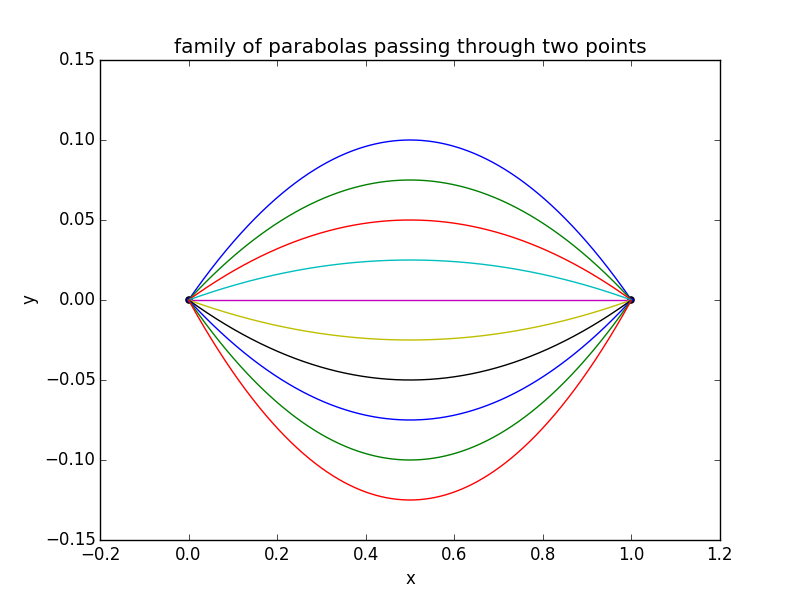
\includegraphics[width=\textwidth]{Files/family_of_curves}
        \caption{Shows how setting up the initial and final points for a curve such as a parabola does not give enough constraints to yield a specific curve. Further information is needed to find a particular parabola among all the possibilities of the family.}
        \label{fig:family of curves}
    \end{figure}

    The goal of the human-robot interaction is to give instructions of a drawing routine that best represents what the user has in mind. The user will therefore have to create a sequence of different curves in an algorithmic way. Each chunk of information will be composed of the initial and final point from which to start and end one curve, and the type of curve. For the simplest types of curves this amount of information will be sufficient, for instance in the straight line case there is only one specific line that passes through 2 distinct points. For more complex curves like circumferences or parabolas, 2 points constrained are not enough to determine one single curve, but rather define a family of curves.\\
    In order to pick the desired curve among all the possible ones the user will be able to visually experiment the change of the free parameter and choose the one curve that best fits his needs (Figure~\ref{fig:family of curves}).

    \begin{figure}
        \centering
        \framebox{\parbox{\textwidth}{\small\tt%
        In [1]: \%run ``/var/folders/7m/g46sl8tx7\_q5dmkzysz8l1640000gn/T/tmpUzITPu.p''\\~\\
        What is the starting point? (Give coordinates): [-1;3]\\~\\
        What is the final point? (Give coordinates): [4;5]\\~\\
        What curve do you want to use?:1. Straight line, 2. Parabola, 3. Circumference, 4. Hyperbola, 5. Sine wave 2\\~\\
        You have selected the curve `parabola'. Additional information is needed. Do you want to specify the vertex of the curve or a third point on the curve? Press 1 for the first option or Press 2 for the second option 2\\~\\
        Please give the coordinates of the specified point: [2,2]\\~\\
        Next curve. What is the starting point? Give coordinates or press Y to choose the end point of the previous curve.%
        }}
        \caption{shows a concept log interface with instructions given to draw a parabola. The output is shown in Figure~\ref{fig:requested curve}}
        \label{fig:log interface}
    \end{figure}
    \begin{figure}
        \centering
        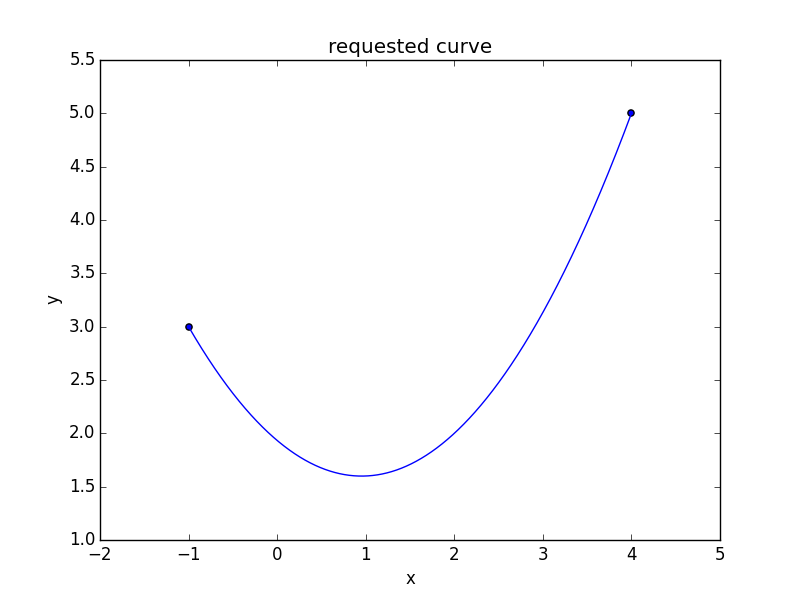
\includegraphics[width=\textwidth]{Files/requested_curve}
        \caption{drawing routine that would be produced by the input of the dialog interface shown in Figure~\ref{fig:log interface}.}
        \label{fig:requested curve}
    \end{figure}


    The interface constitutes the very last step of the project development and the time constraints will probably be too tight for its realisation. There are various steps of complexity that can be pursued, the first one being an implementation of a log dialog that would be likely not to enthusiasm the user especially considering that the target age is childhood. However, this represents the first stage in the interface development and it is a necessary step for the completion of further, more sophisticated milestones that can be accomplished by future groups if the supervision will decide to keep on proposing this project in the next years.\\
    The log dialog would therefore consist of a series of questions that the computer asks the user and it would be based on a cartesian system (Figure~\ref{fig:log interface}\todo{Put the text into that figure}). Each portion of the picture to be generated would require its own set of information that will be composed of the following:
    \begin{enumerate}
        \item What is the starting point? (Give coordinates)
        \item What is the final point? (Give coordinates)
        \item What curve do you want to use?
        \begin{itemize}
            \item Straight line
            \item Parabola
            \item Circumference
            \item Hyperbola
            \item Ellipse
            \item Sine wave
        \end{itemize}
    \end{enumerate}
    Now if the curve requires additional parameters the interface shall ask for additional information, \eg if the option `circumference' is selected, this would be the following question:
    \begin{enumerate}[resume]
        \item You have selected the curve `circumference'. Additional information is needed. Do you want to specify the centre of the circumference or a third point on the curve?
        \begin{itemize}
            \item Press 1 for the first option
            \item Press 2 for the second option
        \end{itemize}
        \item Please give the coordinates of the specified point.
        \item Next curve. What is the starting point? Give coordinates or press Y to choose the end point of the previous curve.
    \end{enumerate}
    In the case of a parabola instead, the coordinates of the vertex would be required, as in the hyperbola case. Obviously the log cannot be an ending point as our target children are very likely to be unfamiliar with Cartesian systems. This would rather serve as a testing version of the future visual interface system.

    \begin{figure}
        \centering
        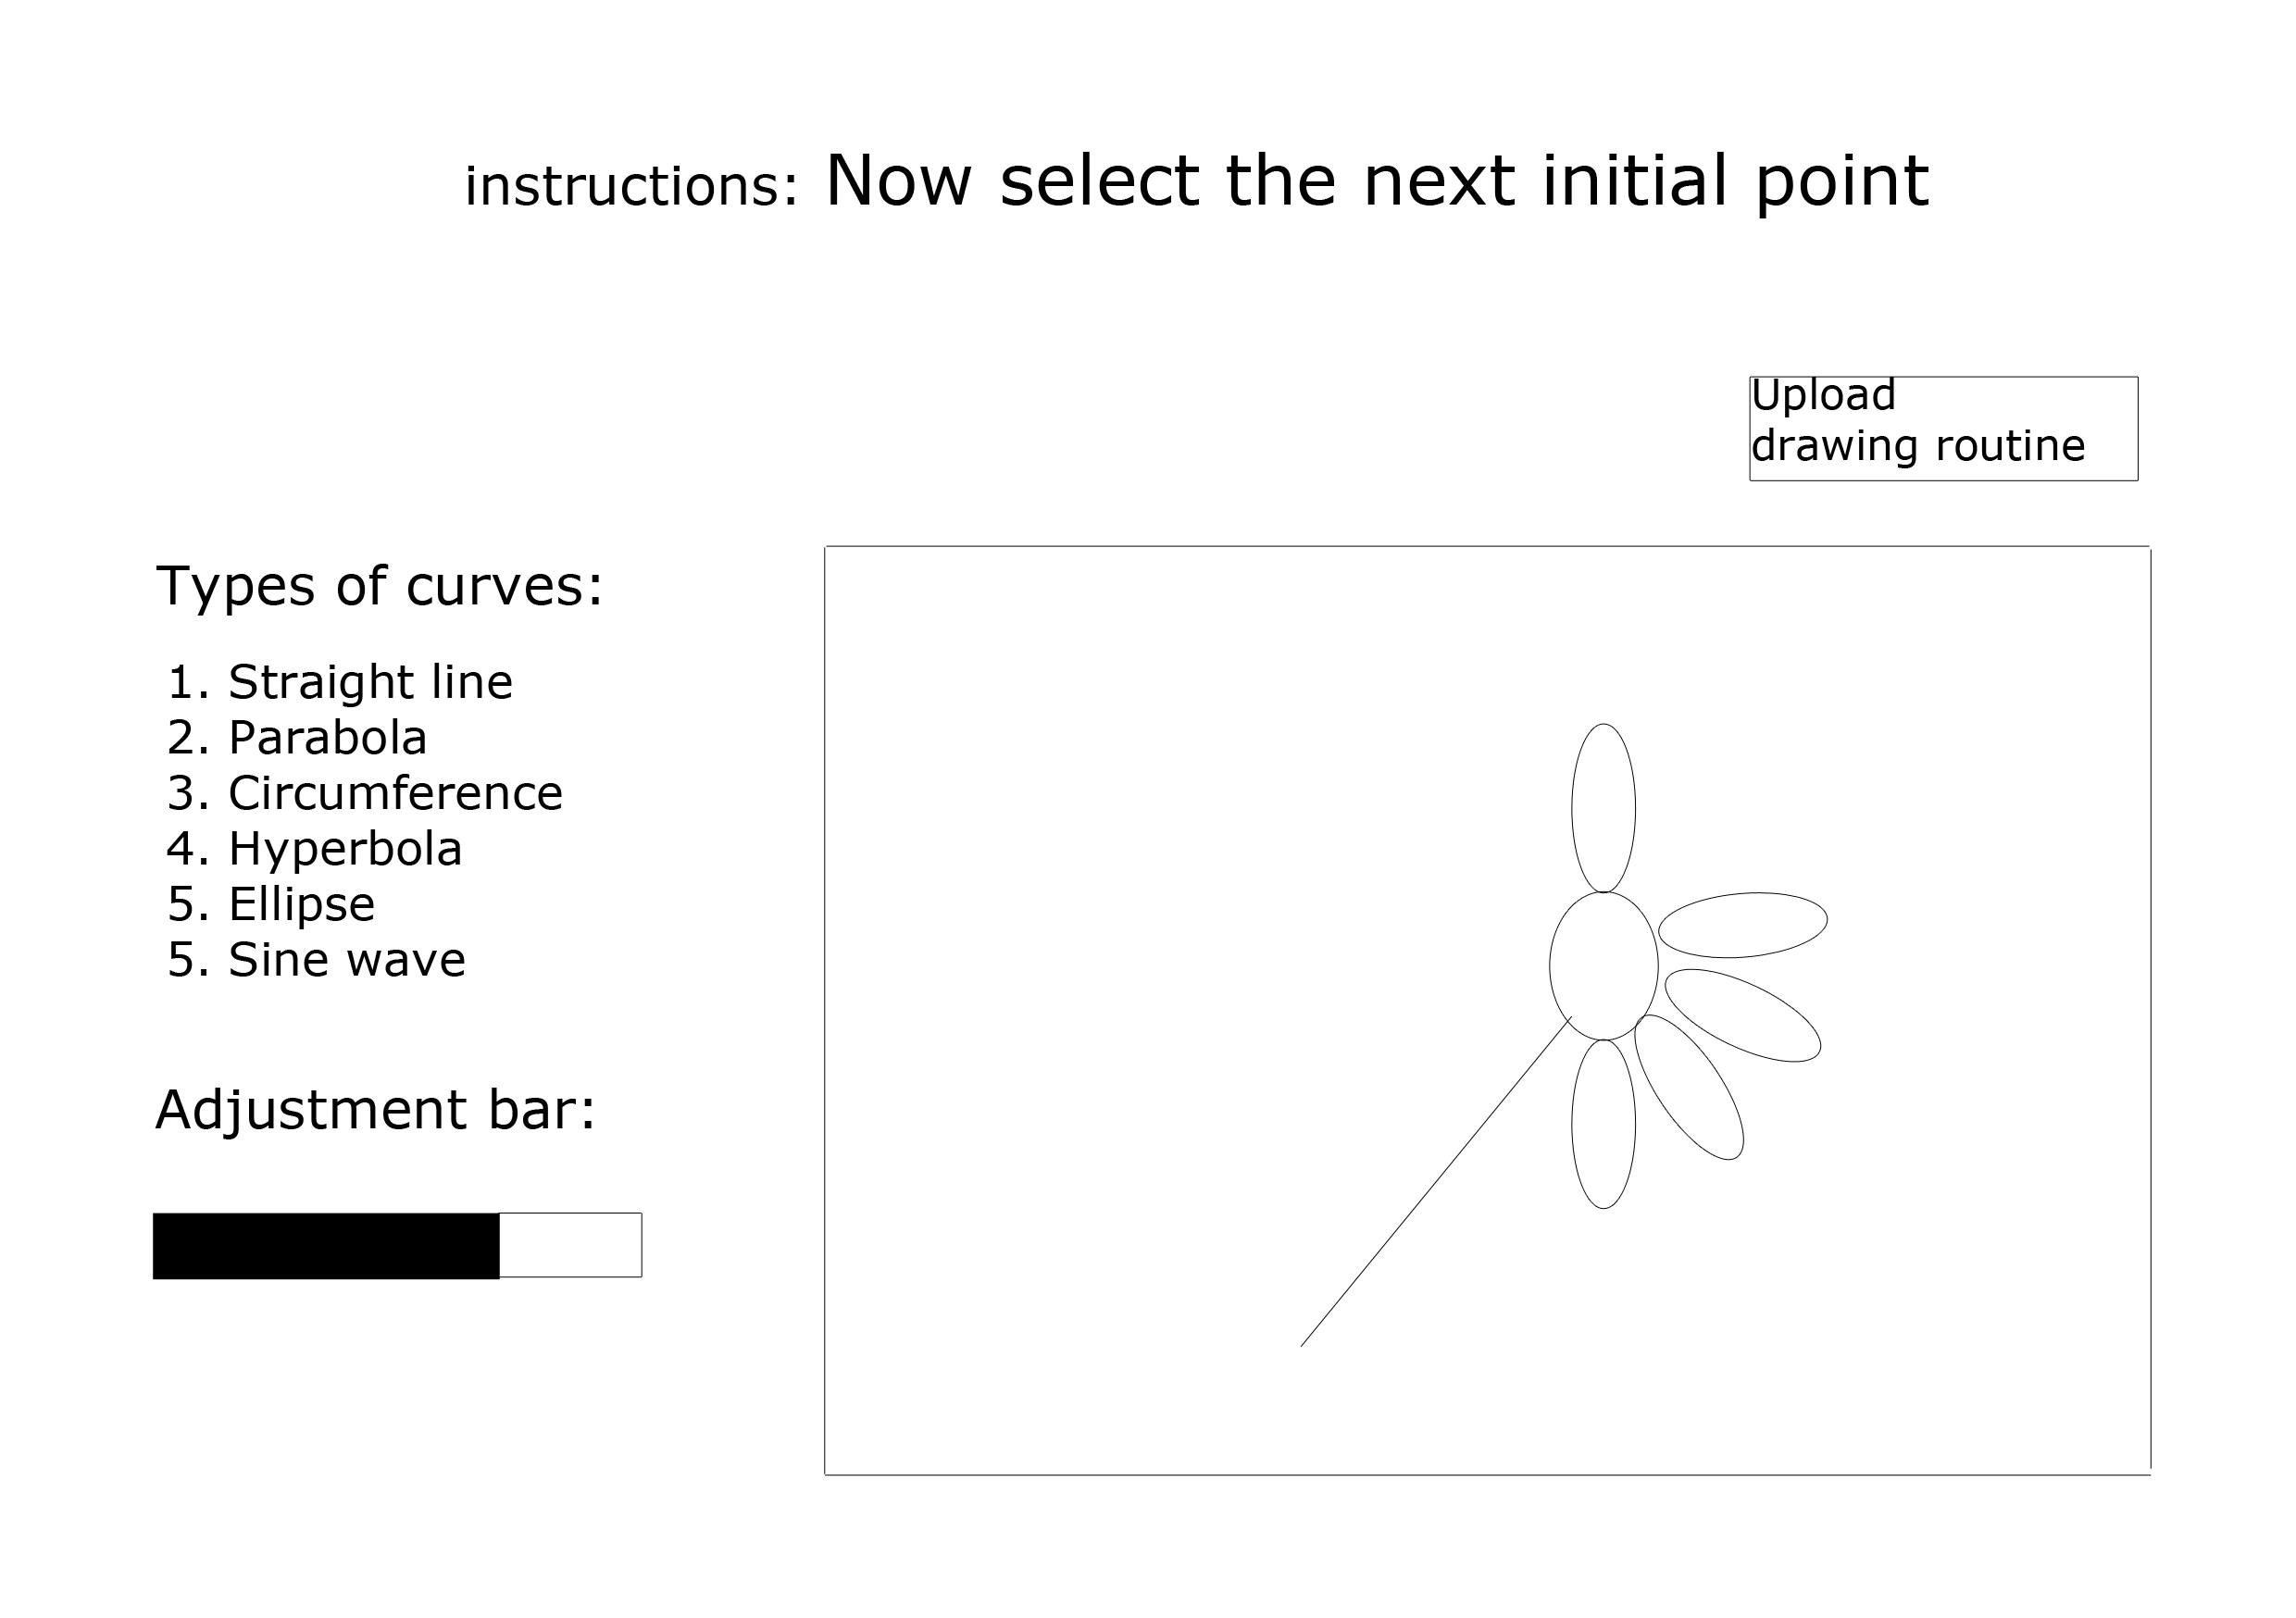
\includegraphics[width=\textwidth]{Files/visual_interface_concept}
        \caption{Concept of a possible user interface for designing routines. In this case the user is trying to draw flower using different geometric figures available. The adjustment bar serves to see the different possible curves that share the same constraints of initial and final points, and choose the one the best fits the needs for the final picture.}
        \label{fig:visual interface concept}
    \end{figure}

    A visual version of the interface would instead consist of a display that shows the input routine while it is being designed. The process would still be consist of step, each of which being a portion of the final overall picture but the input will be given by clicking on the initial and final points and the type of curve will be chosen from a drop-down menu. Most importantly the additional parameter will be determined by choosing a value on an adjustable level bar. When the bar indicator on the bar is moved the displayed curve is instantly displayed with the new parameter, so that the user can see the effect of this changing and therefore choose its value accordingly (Figure~\ref{fig:visual interface concept}).\\
    Once that a routine is completed, the information will be transcribed as a set of rules written in processing, the language read by \gls{Arduino}. Then this code will be transmitted to the robot via a USB cable and the routine will successfully be programmed. The user will have to carefully position the robot at a point that he imagined to be the initial point of the drawing routine, a corner of the drawing rectangle or any other reference point that is indicated by the programmers.

    The transcription of the instructions from the user input to the Arduino language is the main challenge that constitutes the realisation of this part of the project. However Arduino provides with convenient \glspl{library} and the instruction will be transcribed in a consistent way. The \gls{GPS} will monitor the position and the compass will help keeping the right direction. The hardest part is finding the right combination of speeds for the motors attached to the two wheels, that makes it move following a specific shape given by the curve selected by the user.\\
    The main idea is that the traction differential will be proportional to the slope of the curve in the point that is being drawn, and therefore the motor speeds which are controllable in a \numrange{0}{255} range from the Arduino code. This can be intuitively understood upon the consideration that speed is the first derivative of space according to Newton's laws. This problem is solvable both analytically by finding the equations of the derivatives of the curves or computationally by finding the value of the derivative in each point that is needed.\todo{This is far too theoretical for an engineering report: the physics assumes the system is much simpler than it actually is.}

    In the case in which the interface stage will not be reached by the project, which is most probable due to the time constraints that do not allow further work, we hope that the considerations made here will be helpful for future groups in the years to come.
